% ============================================================
%  hw4_sol.tex   --  MATH 6660, Homework 4, Problem 4(a)-(c).
%
%  RULE: nothing in this document goes beyond the class lectures.
%  Every step is tagged with the lecture it comes from.  Anything that
%  would go outside them is wrapped in \outside{}{} and prints as a red
%  labelled box, so it is visible in the PDF.
%
%  Problems 1-3 and 4(d) (the computations) are in hw4_sol_numerical.tex.
%  Build: pdflatex hw4_sol.tex   (twice, for cross-references)
% ============================================================
\documentclass[11pt]{article}
\usepackage[letterpaper,margin=1in]{geometry}
\usepackage[T1]{fontenc}
\usepackage{amsmath,amssymb,amsthm}
\usepackage{booktabs}
\usepackage{array}
\usepackage{graphicx}
\usepackage{caption}
\usepackage{enumitem}
\usepackage{bm}
\usepackage{tikz}
\usepackage{xcolor}
\usepackage[colorlinks=true,linkcolor={blue!45!black},pdfborder={0 0 0}]{hyperref}
\usepackage{pdfcomment}
\usepackage{xspace}

% every figure and table carries a number and sits where it was written
\captionsetup{font=small,labelfont=bf,justification=justified,
              singlelinecheck=false,skip=6pt,hypcap=false}

\newcommand{\dx}{\,\mathrm{d}x}
\newcommand{\dxdy}{\,\mathrm{d}x\,\mathrm{d}y}
\newcommand{\ds}{\,\mathrm{d}s}
\newcommand{\norm}[1]{\lVert #1\rVert}
\newcommand{\abs}[1]{\lvert #1\rvert}
\newcommand{\eps}{\varepsilon}
\newcommand{\ie}{i.e.\@\xspace}
\newcommand{\eg}{e.g.\@\xspace}
\newcommand{\Om}{\Omega}
\newcommand{\dOm}{\partial\Omega}
\newcommand{\grad}{\nabla}
\newcommand{\lap}{\Delta}
\newcommand{\Iint}{\iint_{\Om}}
\newcommand{\Vsp}{V}
\newcommand{\nn}{\bm{n}}
\setlength{\parindent}{0pt}

% ---- provenance tag: which lecture a step comes from ------------------
\newcommand{\src}[1]{{\small\color{black!55}\textsf{[#1]}}}

% ---- anything outside the lectures is boxed and labelled -------------
\newcommand{\outside}[2]{%
  \par\smallskip\noindent
  \fcolorbox{red!65!black}{red!4}{%
    \parbox{0.955\linewidth}{\small
      \textbf{\color{red!65!black}NOT FROM LECTURE --- #1}\par\smallskip #2}}%
  \par\smallskip}

% ---- bullets ---------------------------------------------------------
\newlist{steps}{itemize}{1}
\setlist[steps]{label=\textbullet, leftmargin=1.25em, topsep=3pt,
                itemsep=4pt, parsep=0pt}

% ---- hover tooltips on cross-references ------------------------------
\makeatletter
\newcommand{\settip}[2]{\expandafter\gdef\csname femtip@#1\endcsname{#2}}
\newcommand{\gettip}[1]{%
  \ifcsname femtip@#1\endcsname\csname femtip@#1\endcsname\else equation \ref{#1}\fi}
\newcommand{\eqr}[1]{\pdftooltip{\eqref{#1}}{\gettip{#1}}}
\makeatother

\settip{eq:pde}{Poisson problem: minus the Laplacian of u equals f on the square, u equals g on its boundary}
\settip{eq:ibp}{After the product rule and the divergence theorem: gradient-gradient integral minus the boundary integral of v times the normal derivative equals the load integral}
\settip{eq:weak}{Weak form: the integral of grad u dot grad v equals the integral of f v}
\settip{eq:spaces}{Trial set V_g: finite energy and v equals g on the boundary. Test space V_0: finite energy and v equals 0 on the boundary}
\settip{eq:lifted}{Lifted problem: B(w,v) equals L-tilde(v) for all v in V_0, with u = w + G}
\settip{eq:poinc}{Poincare on the square: the L2 norm squared of v is at most 4 times the L2 norm squared of grad v}
\settip{eq:ke}{Element stiffness matrix of the bilinear square, one sixth of 4,-1,-2,-1 and its cyclic shifts}
\settip{eq:row}{Assembled equation for interior node (i,j): one third of 8 U_ij minus its eight neighbours equals b_ij}
\settip{eq:shapes}{The four bilinear shape functions, (1-xi)(1-eta), xi(1-eta), xi eta, (1-xi) eta}

\begin{document}

\begin{center}
  {\large\bfseries MATH 6660 --- Homework 4}\\[2pt]
  {\normalsize 2D Cartesian FEM, Problem 4(a)--(c)}\\[2pt]
  {\small Fall 2026}
\end{center}

\vspace{4pt}

{\small\color{black!60}
\textbf{Relation to the lectures.}  Lecture 13, Part III, does exactly this
problem with $u=0$ on $\dOm$: product rule, divergence theorem, $V=H^{1}_{0}$,
and the four Lax--Milgram checks with a Poincar\'e constant left unnamed.  Two
things change here.  The boundary value is $g\neq0$, which is Lecture 5's
nonhomogeneous Dirichlet case (trial set $\neq$ test space, lifting).  And the
elements are squares with the bilinear interpolant the problem gives; their
basis turns out to be products of Lecture 4's 1D hats.  The Poincar\'e
constant for the square is computed by Lecture 8's 1D argument.}

\vspace{4pt}

% ==================================================================
\section*{Problem 4(a)}

\textbf{Problem.} Recast this problem as a variational problem.  Clearly state
the test and trial function spaces.

\medskip
The strong problem is
\begin{equation}\label{eq:pde}
  -\grad\cdot\grad u=-u_{,xx}-u_{,yy}=f(x,y)\quad\text{in } \Om=(-1,1)\times(-1,1),
  \qquad u=g\quad\text{on } \dOm .
\end{equation}

% ------------------------------------------------------------------
\subsection*{Step 1 --- multiply by $v$, integrate, move one derivative
  \ \src{Lecture 13, Part III: product rule, then divergence theorem}}

\begin{steps}
\item Multiply \eqr{eq:pde} by a test function $v$ and integrate over $\Om$:
\begin{equation}\label{eq:mult}
  -\Iint v\,\lap u\dxdy=\Iint f v\dxdy .
\end{equation}
\item Product rule, $\grad\cdot(v\grad u)=\grad v\cdot\grad u+v\,\lap u$, so the
      left side of \eqref{eq:mult} is
\begin{equation}\label{eq:prod}
  -\Iint v\,\lap u\dxdy=\Iint\grad u\cdot\grad v\dxdy-\Iint\grad\cdot(v\grad u)\dxdy .
\end{equation}
\item Divergence theorem on the last term, $\nn$ the outward unit normal:
      $\Iint\grad\cdot(v\grad u)\dxdy=\oint_{\dOm}v\,\grad u\cdot\nn\ds$.  Put
      this into \eqref{eq:prod} and \eqref{eq:prod} into \eqref{eq:mult}:
\begin{equation}\label{eq:ibp}
  \Iint\grad u\cdot\grad v\dxdy
  \;-\;\oint_{\dOm}v\,\underbrace{\grad u\cdot\nn}_{\text{normal flux, not given}}\ds
  \;=\;\Iint f v\dxdy .
\end{equation}
\end{steps}

% ------------------------------------------------------------------
\subsection*{Step 2 --- kill the boundary term
  \ \src{Lecture 5: Dirichlet $=$ essential, the test function vanishes there}}

\begin{steps}
\item On all four sides the data is the \emph{value} $u=g$.  The flux
      $\grad u\cdot\nn$ there is not known --- it is the reaction to holding $u$
      at $g$.  So the boundary integral in \eqr{eq:ibp} cannot be evaluated.
\item The only way to remove it is to demand $v=0$ on $\dOm$.  Then
      \eqr{eq:ibp} becomes
\begin{equation}\label{eq:weak}
  \boxed{\;\Iint\grad u\cdot\grad v\dxdy=\Iint f v\dxdy\;}
\end{equation}
\end{steps}

% ------------------------------------------------------------------
\subsection*{Step 3 --- the trial set and the test space
  \ \src{Lecture 5: $u(0)=\alpha\neq0$ gives trial $\Vsp\neq$ test $\Vsp_{0}$;
         Lecture 13, eq.~(1.254), for the 2D integrals}}

\begin{steps}
\item \eqr{eq:weak} needs $\Iint\abs{\grad u}^{2}$ and $\Iint\abs{\grad v}^{2}$
      finite, so both spaces are built on
      $\Iint\bigl[v^{2}+\abs{\grad v}^{2}\bigr]\dxdy<\infty$, as in Lecture 13.
\item The unknown $u$ must also satisfy the essential condition $u=g$; the
      test function must satisfy $v=0$ (Step 2):
\begin{equation}\label{eq:spaces}
  \boxed{\;
  \begin{aligned}
  \text{trial: }\ V_{g}&=\Bigl\{v:\ \Iint\bigl[v^{2}+\abs{\grad v}^{2}\bigr]\dxdy<\infty,
       \ \ v=g \text{ on } \dOm\Bigr\},\\
  \text{test: }\ V_{0}&=\Bigl\{v:\ \Iint\bigl[v^{2}+\abs{\grad v}^{2}\bigr]\dxdy<\infty,
       \ \ v=0 \text{ on } \dOm\Bigr\}=H^{1}_{0}(\Om),
  \end{aligned}\;}
\end{equation}
      with $\abs{\grad v}^{2}=(v_{,x})^{2}+(v_{,y})^{2}$.
\item They differ because $g\neq0$ (in part (d), $g=1$).  Exactly Lecture 5's
      warning: $V_{g}$ is not a vector space --- $u_{1}+u_{2}$ has boundary
      value $2g$ --- while $V_{0}$ is.
\end{steps}

\medskip
\noindent\fbox{\parbox{0.955\linewidth}{%
\textbf{(Variational problem)}\ \ Find $u\in V_{g}$ such that
\[
  \Iint\grad u\cdot\grad v\dxdy=\Iint f v\dxdy
  \qquad\text{for all } v\in V_{0},
\]
with trial set $V_{g}$ and test space $V_{0}=H^{1}_{0}(\Om)$ from \eqr{eq:spaces}.}}

\medskip
{\small\color{black!60}\textbf{Mechanics reading.}  A membrane with unit tension
under pressure $f$, its rim held at height $g$.  $V_{g}$: deflected shapes that
honour the rim.  $V_{0}$: virtual deflections, which may not move the rim.
\eqr{eq:weak} is virtual work; the rim reaction does no virtual work because
$v=0$ there.}

% ==================================================================
\newpage
\section*{Problem 4(b)}

\textbf{Problem.} Show that the variational problem has a unique solution by
showing that it meets all of the criteria of the Lax--Milgram theorem.

% ------------------------------------------------------------------
\subsection*{Step 1 --- put the problem in Lax--Milgram's form
  \ \src{Lecture 13: $u$ and $v$ in the same Hilbert space;
         Lecture 5: lift the boundary data}}

\begin{steps}
\item Lax--Milgram (Lecture 13) asks for \emph{one} Hilbert space $\Vsp$ with
      $u,v\in\Vsp$.  In 4(a), $u\in V_{g}$ but $v\in V_{0}$.  Lecture 5's fix:
      split off a known function that carries the boundary data.
\item Pick any $G\in V_{g}$.  (If $V_{g}$ were empty there would be no
      candidate $u$ at all.)  For part (d), $g=1$ and $G\equiv1$ works:
      $\Iint[1^{2}+0]\dxdy=4<\infty$.
\item Write $u=w+G$.  Then $w=g-g=0$ on $\dOm$, so $w\in V_{0}$.  Substitute in
      \eqr{eq:weak} and move the known part to the right:
\begin{equation}\label{eq:lifted}
  \underbrace{\Iint\grad w\cdot\grad v\dxdy}_{B(w,v)}
  \;=\;\underbrace{\Iint f v\dxdy-\Iint\grad G\cdot\grad v\dxdy}_{\widetilde{L}(v)}
  \qquad\forall\,v\in\Vsp:=V_{0}=H^{1}_{0}(\Om),
\end{equation}
      with the norm of Lecture 13,
      $\norm{v}^{2}_{\Vsp}=\norm{v}^{2}+\norm{\grad v}^{2}$, where
      $\norm{\cdot}$ is the $L^{2}(\Om)$ norm.
\end{steps}

% ------------------------------------------------------------------
\subsection*{Step 2 --- (S) and (CB)
  \ \src{Lecture 13, Part III, checks 1--2; Lecture 6: Cauchy}}

\begin{steps}
\item \textbf{(S)} $\grad w\cdot\grad v=\grad v\cdot\grad w$ pointwise, so
      $B(w,v)=B(v,w)$.
\item \textbf{(CB)}
\begin{equation}\label{eq:cb}
  \abs{B(w,v)}
  \le\underbrace{\Iint\abs{\grad w}\,\abs{\grad v}\dxdy}_{\abs{\bm a\cdot\bm b}\le\abs{\bm a}\abs{\bm b}}
  \le\underbrace{\norm{\grad w}\,\norm{\grad v}}_{\text{Cauchy}}
  \le\underbrace{\norm{w}_{\Vsp}\norm{v}_{\Vsp}}_{\norm{\grad v}^{2}\le\norm{v}^{2}+\norm{\grad v}^{2}},
  \qquad\beta^{*}=1 .
\end{equation}
\end{steps}

% ------------------------------------------------------------------
\subsection*{Step 3 --- Poincar\'e on the square
  \ \src{Lecture 8, eqs.~(1.127)--(1.128): the same three lines, in $x$, for
         each fixed $y$}}

\begin{steps}
\item Take $v\in V_{0}$ and fix $y$.  $v(-1,y)=0$ on the left side, so
\begin{equation}\label{eq:p1}
  v(x,y)=\int_{-1}^{x}v_{,x}(s,y)\,\mathrm{d}s .
\end{equation}
\item Bound it by the whole line and apply Cauchy to $1\cdot\abs{v_{,x}}$ on an
      interval of length $2$:
\begin{equation}\label{eq:p2}
  \abs{v(x,y)}\le\int_{-1}^{1}\abs{v_{,x}(s,y)}\,\mathrm{d}s
  \le\underbrace{\Bigl(\int_{-1}^{1}1^{2}\,\mathrm{d}s\Bigr)^{1/2}}_{\sqrt2}
     \Bigl(\int_{-1}^{1}v_{,x}(s,y)^{2}\,\mathrm{d}s\Bigr)^{1/2} .
\end{equation}
\item Square \eqref{eq:p2}.  The right side no longer depends on $x$, so
      integrating over $x\in(-1,1)$ multiplies it by $2$; then integrate over
      $y\in(-1,1)$:
\begin{equation}\label{eq:poinc}
  \boxed{\;\norm{v}^{2}=\Iint v^{2}\dxdy\le
  \underbrace{2\cdot2}_{x\text{-length}\,\times\,\eqref{eq:p2}}\Iint(v_{,x})^{2}\dxdy
  \le4\,\norm{\grad v}^{2}\;}
\end{equation}
      This is Lecture 13's multi-dimensional Poincar\'e,
      $\norm{v}\le C\norm{\grad v}$, with $C=2$.
\end{steps}

% ------------------------------------------------------------------
\subsection*{Step 4 --- (VE) and the bound on $\widetilde{L}$
  \ \src{Lecture 13, Part III, checks 3--4}}

\begin{steps}
\item \textbf{(VE)} Split $B(v,v)$ in half and use \eqr{eq:poinc} on one half:
\begin{equation}\label{eq:ve}
  B(v,v)=\norm{\grad v}^{2}
  =\tfrac12\norm{\grad v}^{2}+\underbrace{\tfrac12\norm{\grad v}^{2}}_{\ge\,\frac18\norm{v}^{2}\ \text{by \eqr{eq:poinc}}}
  \ge\tfrac18\bigl(\norm{\grad v}^{2}+\norm{v}^{2}\bigr)
  =\tfrac18\norm{v}^{2}_{\Vsp},
  \qquad\beta_{*}=\tfrac18 .
\end{equation}
      Same as Lecture 13's $\beta_{*}=\tfrac12\min(1/C^{2},1)$ with $C=2$.
\item \textbf{$\widetilde{L}$ bounded}, by Cauchy on each term of
      \eqr{eq:lifted}:
\begin{equation}\label{eq:lb}
  \abs{\widetilde{L}(v)}\le\norm{f}\,\norm{v}+\norm{\grad G}\,\norm{\grad v}
  \le\bigl(\norm{f}+\norm{\grad G}\bigr)\norm{v}_{\Vsp} .
\end{equation}
      This needs $\Iint f^{2}<\infty$.  In part (d), $f$ is continuous on the
      closed square, $e^{\sin\pi x\sin\pi y}\le e$ and the brace is at most
      $2+2+1+1=6$, so $\abs{f}\le6\pi^{2}e$; and $\grad G=0$.
\end{steps}

\begin{center}
\begin{minipage}{\linewidth}
\centering\small
\renewcommand{\arraystretch}{1.25}
\begin{tabular}{@{}llll@{}}
\toprule
condition & holds because & constant & equation\\
\midrule
(S)  symmetric          & $\grad w\cdot\grad v=\grad v\cdot\grad w$ & --- & Step 2\\
(CB) bounded            & Cauchy                                   & $\beta^{*}=1$ & \eqref{eq:cb}\\
(VE) $\Vsp$-elliptic    & Poincar\'e, $C=2$                        & $\beta_{*}=1/8$ & \eqref{eq:ve}\\
$\widetilde{L}$ bounded & Cauchy                                   & $\norm{f}+\norm{\grad G}$ & \eqref{eq:lb}\\
\bottomrule
\end{tabular}
\captionof{table}{The four Lax--Milgram conditions for \eqr{eq:lifted} on
$\Vsp=H^{1}_{0}\bigl((-1,1)^{2}\bigr)$.}
\label{tab:lm}
\end{minipage}
\end{center}

% ------------------------------------------------------------------
\subsection*{Step 5 --- conclusion, and uniqueness of $u$ itself}

\begin{steps}
\item Table~\ref{tab:lm} meets every hypothesis of Lax--Milgram, so
      \eqr{eq:lifted} has a unique $w\in V_{0}$, with
      $\norm{w}_{\Vsp}\le\widetilde{L}/\beta_{*}=8\bigl(\norm{f}+\norm{\grad G}\bigr)$.
      Then $u=w+G\in V_{g}$ solves the variational problem of 4(a).
\item $u$ does not depend on which $G$ was picked.  If $u_{1},u_{2}\in V_{g}$
      both solve it, $d=u_{1}-u_{2}$ has boundary value $g-g=0$, so
      $d\in V_{0}$, and subtracting the two problems gives $B(d,v)=0$ for all
      $v\in V_{0}$.  Take $v=d$ and use \eqr{eq:ve}:
\begin{equation}\label{eq:uniq}
  \tfrac18\norm{d}^{2}_{\Vsp}\le B(d,d)=0
  \qquad\Longrightarrow\qquad d=0,\ \ u_{1}=u_{2}.
\end{equation}
\end{steps}

\medskip
\noindent\fbox{\parbox{0.955\linewidth}{%
\textbf{Conclusion.}  With $u=w+G$, the problem for $w$ on $H^{1}_{0}(\Om)$
satisfies (S), (CB) with $\beta^{*}=1$, (VE) with $\beta_{*}=1/8$, and
$\widetilde{L}$ is bounded.  By Lax--Milgram the variational problem of 4(a)
has exactly one solution $u\in V_{g}$.}}

\medskip
{\small\color{black!60}\textbf{Mechanics reading.}  (VE) is ``no rigid-body
mode'': the rim is held, so a membrane cannot move without stretching.
\eqr{eq:poinc} is the 2D version of Lecture 8's ``pinned ends cannot move for
free'' --- held on the left side, a deflection is controlled by its slope.
$\beta^{*}/\beta_{*}=8$ is the constant that C\'ea's lemma will carry into the
error estimate of part (d).}

% ==================================================================
\newpage
\section*{Problem 4(c)}

\textbf{Problem.} Develop a finite element method for this problem based on
square elements.  On each element the solution on the four corners is
interpolated with $s(x,y)=\alpha_{1}+\alpha_{2}x+\alpha_{3}y+\alpha_{4}xy$.
Write out the basis functions and explicitly write out the linear system
(uniform grid, same spacing in $x$ and $y$).

% ------------------------------------------------------------------
\subsection*{Step 1 --- grid, element, local coordinates}

\begin{steps}
\item $N\times N$ squares, $h=2/N$, nodes $x_{i}=-1+ih$, $y_{j}=-1+jh$,
      $i,j=0,\dots,N$.  Interior nodes $1\le i,j\le N-1$: $(N-1)^{2}$ unknowns.
      Boundary nodes carry the known value $g(x_{i},y_{j})$.
\item Element $K_{ij}=[x_{i},x_{i+1}]\times[y_{j},y_{j+1}]$, local coordinates
      $\xi=(x-x_{i})/h$, $\eta=(y-y_{j})/h\in[0,1]$, corners numbered
      counter-clockwise from $(x_{i},y_{j})$ (Figure~\ref{fig:element}).
\end{steps}

% ------------------------------------------------------------------
\subsection*{Step 2 --- the four corner values fix $s$; the shape functions}

\begin{steps}
\item Put $x=x_{i}+h\xi$, $y=y_{j}+h\eta$ into $s$ and collect powers:
\begin{equation}\label{eq:sloc}
  s=\underbrace{\alpha_{1}+\alpha_{2}x_{i}+\alpha_{3}y_{j}+\alpha_{4}x_{i}y_{j}}_{c_{1}}
   +\underbrace{h(\alpha_{2}+\alpha_{4}y_{j})}_{c_{2}}\,\xi
   +\underbrace{h(\alpha_{3}+\alpha_{4}x_{i})}_{c_{3}}\,\eta
   +\underbrace{h^{2}\alpha_{4}}_{c_{4}}\,\xi\eta .
\end{equation}
      Read bottom-up, $\alpha_{4},\alpha_{3},\alpha_{2},\alpha_{1}$ follow from
      $c_{4},c_{3},c_{2},c_{1}$ one at a time, so the $\alpha$'s and the $c$'s
      carry the same information.
\item Evaluate \eqref{eq:sloc} at the four corners, $s_{1}=s(0,0)$,
      $s_{2}=s(1,0)$, $s_{3}=s(1,1)$, $s_{4}=s(0,1)$:
      $s_{1}=c_{1}$, $s_{2}=c_{1}+c_{2}$, $s_{4}=c_{1}+c_{3}$,
      $s_{3}=c_{1}+c_{2}+c_{3}+c_{4}$.  Solved one at a time,
\begin{equation}\label{eq:cs}
  c_{1}=s_{1},\quad c_{2}=s_{2}-s_{1},\quad c_{3}=s_{4}-s_{1},\quad
  c_{4}=s_{3}-s_{2}-s_{4}+s_{1},
\end{equation}
      a unique interpolant for any four corner values.
\item Put \eqref{eq:cs} back into \eqref{eq:sloc} and collect by corner value:
      $s=\sum_{a=1}^{4}s_{a}N_{a}(\xi,\eta)$ with
\begin{equation}\label{eq:shapes}
  \boxed{\;N_{1}=(1-\xi)(1-\eta),\qquad N_{2}=\xi(1-\eta),\qquad
          N_{3}=\xi\eta,\qquad N_{4}=(1-\xi)\eta\;}
\end{equation}
      Each is $1$ at its own corner and $0$ at the other three.
\end{steps}

\begin{center}
\begin{minipage}{\linewidth}
\centering
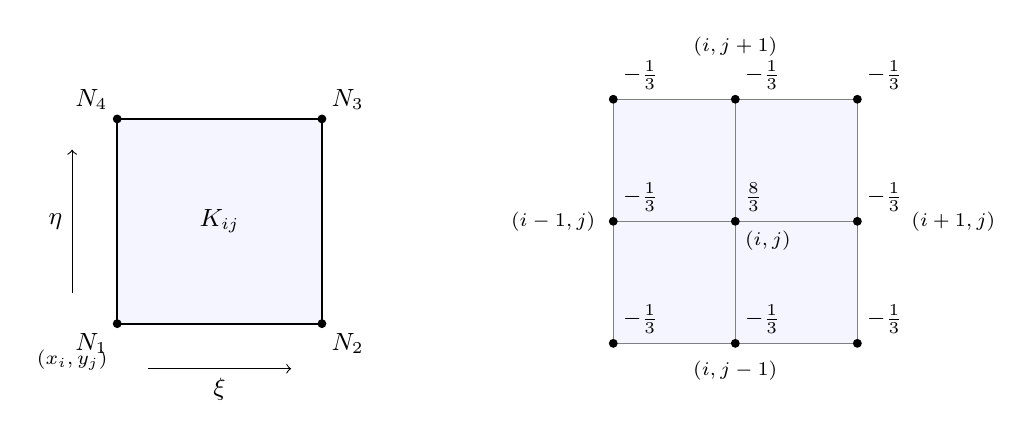
\begin{tikzpicture}[font=\small]
  % one element
  \begin{scope}[x=2.6cm,y=2.6cm]
    \draw[thick,fill=blue!4] (0,0) rectangle (1,1);
    \foreach \x/\y/\n/\pos in {0/0/1/below left,1/0/2/below right,1/1/3/above right,0/1/4/above left}
      {\fill (\x,\y) circle (1.6pt); \node[\pos] at (\x,\y) {$N_{\n}$};}
    \node at (0.5,0.5) {$K_{ij}$};
    \draw[->] (0.15,-0.22) -- (0.85,-0.22) node[midway,below] {$\xi$};
    \draw[->] (-0.22,0.15) -- (-0.22,0.85) node[midway,left] {$\eta$};
    \node[font=\scriptsize,below left] at (0,-0.08) {$(x_{i},y_{j})$};
  \end{scope}
  % the four elements around node (i,j)
  \begin{scope}[x=1.55cm,y=1.55cm,xshift=6.3cm,yshift=-0.25cm]
    \fill[blue!4] (0,0) rectangle (2,2);
    \foreach \t in {0,1,2}{\draw[gray] (\t,0) -- (\t,2); \draw[gray] (0,\t) -- (2,\t);}
    \foreach \x in {0,1,2}{\foreach \y in {0,1,2}{\fill (\x,\y) circle (1.6pt);}}
    \foreach \x/\y in {0/0,1/0,2/0,0/1,2/1,0/2,1/2,2/2}
      {\node[font=\footnotesize,above right=0pt] at (\x,\y) {$-\tfrac13$};}
    \node[font=\footnotesize,above right=0pt] at (1,1) {$\tfrac83$};
    \node[font=\scriptsize,below=3pt] at (1,0) {$(i,j-1)$};
    \node[font=\scriptsize,below right=0pt] at (1,1) {$(i,j)$};
    \node[font=\scriptsize,above=12pt] at (1,2) {$(i,j+1)$};
    \node[font=\scriptsize,left=3pt] at (0,1) {$(i-1,j)$};
    \node[font=\scriptsize,right=16pt] at (2,1) {$(i+1,j)$};
  \end{scope}
\end{tikzpicture}
\captionof{figure}{Left: one element and its four shape functions
\eqr{eq:shapes}.  Right: the four elements around an interior node $(i,j)$ ---
the support of $\varphi_{ij}$ --- with the coefficients of its row of the
stiffness matrix, \eqr{eq:row}.}
\label{fig:element}
\end{minipage}
\end{center}

% ------------------------------------------------------------------
\subsection*{Step 3 --- continuity, and the global basis
  \ \src{Lecture 4: 1D hats; HW3 Problem 3: a jump puts a delta in the
         derivative}}

\begin{steps}
\item On the right edge of $K_{ij}$, $\xi=1$ and \eqref{eq:shapes} gives
      $s=s_{2}(1-\eta)+s_{3}\eta$: only the two corner values on that edge
      enter.  The neighbour $K_{i+1,j}$ produces the same line from the same
      two values on its left edge.  So $s$ is continuous across every edge,
      $\grad s$ has no delta, $\Iint\abs{\grad s}^{2}<\infty$: the method is
      \textbf{conforming}, $V_{h}\subset$ the spaces of \eqr{eq:spaces}.
\item Glue the $N_{a}$ of the four squares around node $(i,j)$ (Figure
      \ref{fig:element}, right).  On $K_{ij}$ the node is corner $1$, value
      $(1-\xi)(1-\eta)$; on $K_{i-1,j}$ it is corner $2$, value $\xi(1-\eta)$;
      and so on.  In every case the $x$-factor is Lecture 4's hat $\varphi_{i}$
      on the $x$-grid and the $y$-factor is $\varphi_{j}$ on the $y$-grid:
\begin{equation}\label{eq:basis}
  \boxed{\;\varphi_{ij}(x,y)=\varphi_{i}(x)\,\varphi_{j}(y),\qquad
  \varphi_{i}(x)=\begin{cases}1-\abs{x-x_{i}}/h, & \abs{x-x_{i}}\le h,\\
                              0, & \text{otherwise.}\end{cases}\;}
\end{equation}
\item Trial and test functions, with the boundary values as Lecture 5's lift:
\begin{equation}\label{eq:trial}
  U=\underbrace{\sum_{(k,l)\in\dOm}g(x_{k},y_{l})\,\varphi_{kl}}_{\text{known, carries }u=g}
   +\sum_{i,j=1}^{N-1}\xi_{ij}\,\varphi_{ij},
  \qquad v=\varphi_{ij},\ \ 1\le i,j\le N-1 .
\end{equation}
\end{steps}

\medskip
\noindent\fbox{\parbox{0.955\linewidth}{%
\textbf{(FEM)}\ \ Find $U$ of the form \eqr{eq:trial} such that
$\displaystyle\Iint\grad U\cdot\grad\varphi_{ij}\dxdy=\Iint f\varphi_{ij}\dxdy$
for every interior node $(i,j)$.}}

% ------------------------------------------------------------------
\subsection*{Step 4 --- the element stiffness matrix}

\begin{steps}
\item $\partial/\partial x=(1/h)\,\partial/\partial\xi$,
      $\partial/\partial y=(1/h)\,\partial/\partial\eta$ and
      $\mathrm{d}x\,\mathrm{d}y=h^{2}\,\mathrm{d}\xi\,\mathrm{d}\eta$, so
\begin{equation}\label{eq:kedef}
  k^{e}_{ab}=\iint_{K}\grad N_{a}\cdot\grad N_{b}\dxdy
  =\underbrace{\tfrac{1}{h^{2}}\cdot h^{2}}_{=\,1}
   \int_{0}^{1}\!\!\int_{0}^{1}\bigl(N_{a,\xi}N_{b,\xi}+N_{a,\eta}N_{b,\eta}\bigr)
   \,\mathrm{d}\xi\,\mathrm{d}\eta .
\end{equation}
      $h$ cancels: in 2D the stiffness of a square does not depend on its
      size.
\item Every $N_{a}$ in \eqr{eq:shapes} is a product of $1-\xi$ or $\xi$ with
      $1-\eta$ or $\eta$, so \eqref{eq:kedef} splits into 1D integrals:
\begin{equation}\label{eq:1d}
  \int_{0}^{1}(1-\xi)^{2}\mathrm{d}\xi=\tfrac13,\quad
  \int_{0}^{1}\xi(1-\xi)\,\mathrm{d}\xi=\tfrac12-\tfrac13=\tfrac16,\quad
  \bigl[(1-\xi)'\bigr]^{2}=1,\quad (1-\xi)'\,\xi'=-1 .
\end{equation}
\item Three kinds of pair, each ``$x$-part $\times$ $y$-part $+$ $y$-part
      $\times$ $x$-part'':
\begin{equation}\label{eq:kecases}
  \underbrace{1\cdot\tfrac13+\tfrac13\cdot1=\tfrac46}_{a=b},\qquad
  \underbrace{(-1)\cdot\tfrac13+\tfrac16\cdot1=-\tfrac16}_{a,b\ \text{share an edge}},\qquad
  \underbrace{(-1)\cdot\tfrac16+\tfrac16\cdot(-1)=-\tfrac26}_{a,b\ \text{opposite}},
\end{equation}
\begin{equation}\label{eq:ke}
  \boxed{\;\bm{k}^{e}=\frac16\begin{bmatrix}
     4&-1&-2&-1\\ -1&4&-1&-2\\ -2&-1&4&-1\\ -1&-2&-1&4\end{bmatrix}\;}
\end{equation}
      Each row sums to $0$: a constant has no gradient, hence no energy.
\end{steps}

% ------------------------------------------------------------------
\subsection*{Step 5 --- the linear system
  \ \src{Lecture 13, eq.~(1.236): $A_{ij}=B(\varphi_{i},\varphi_{j})$;
         Lecture 5, eq.~(1.66): known values to the RHS; Lecture 4: trapezoidal load}}

\begin{steps}
\item \textbf{Row of an interior node $(i,j)$.}  It sits in $4$ squares as a
      corner, shares each edge-neighbour with $2$ squares and each diagonal
      neighbour with $1$.  From \eqref{eq:kecases}:
      $4\cdot\tfrac46=\tfrac83$, \ $2\cdot(-\tfrac16)=-\tfrac13$, \
      $1\cdot(-\tfrac26)=-\tfrac13$:
\begin{equation}\label{eq:row}
  \boxed{\;\frac13\Bigl[\,8\,U_{i,j}-\sum_{(k,l)\in\mathcal{N}_{ij}}U_{k,l}\Bigr]=b_{ij},
  \qquad 1\le i,j\le N-1,\;}
\end{equation}
      $\mathcal{N}_{ij}$ the eight neighbours $k\in\{i-1,i,i+1\}$,
      $l\in\{j-1,j,j+1\}$, $(k,l)\neq(i,j)$,
      and $U_{k,l}=g(x_{k},y_{l})$ whenever $(k,l)$ is a boundary node.
\item \textbf{Load.}  $b_{ij}=\Iint f\varphi_{ij}$.  The trapezoidal rule of
      Lecture 4 on each square, $\iint_{K}F\approx\tfrac{h^{2}}{4}\sum_{\text{corners}}F$,
      sees $f\varphi_{ij}$ only at corner $(i,j)$, where $\varphi_{ij}=1$; four
      squares:
\begin{equation}\label{eq:load}
  b_{ij}\approx4\cdot\tfrac{h^{2}}{4}\,f(x_{i},y_{j})=h^{2}f_{ij} .
\end{equation}
\item \textbf{Matrix form.}  Order the unknowns row by row,
      $\bm{U}=(U_{1,1},\dots,U_{N-1,1},\,U_{1,2},\dots,U_{N-1,N-1})^{T}$.  Move
      every boundary value in \eqr{eq:row} to the right:
\begin{equation}\label{eq:system}
  \boxed{\begin{gathered}
  \bm{A}\,\bm{U}=\bm{b}+\bm{r},\qquad
  \bm{A}=\frac13\begin{bmatrix}
    \bm{T}&\bm{S}&&\\ \bm{S}&\bm{T}&\ddots&\\ &\ddots&\ddots&\bm{S}\\ &&\bm{S}&\bm{T}
  \end{bmatrix},\\[6pt]
  \bm{T}=\begin{bmatrix}8&-1&&\\-1&8&\ddots&\\&\ddots&\ddots&-1\\&&-1&8\end{bmatrix},\qquad
  \bm{S}=\begin{bmatrix}-1&-1&&\\-1&-1&\ddots&\\&\ddots&\ddots&-1\\&&-1&-1\end{bmatrix}
  \end{gathered}}
\end{equation}
      $\bm{A}$ is $(N-1)^{2}\times(N-1)^{2}$, made of $N-1$ block rows;
      $\bm{T},\bm{S}$ are $(N-1)\times(N-1)$; $\bm{T}$ couples a node to its
      own grid row, $\bm{S}$ to the rows above and below.
\item $r_{ij}=\tfrac13\sum g(x_{k},y_{l})$ over the boundary nodes among the
      eight neighbours of $(i,j)$.  For $g=1$ (part (d)):
\begin{equation}\label{eq:r}
  r_{ij}=\begin{cases}
   5/3, & (i,j)\ \text{next to a corner (5 boundary neighbours)},\\
   1,   & (i,j)\ \text{next to one side (3 boundary neighbours)},\\
   0,   & \text{otherwise}.\end{cases}
\end{equation}
\item $\bm{A}$ is symmetric positive definite by Lecture 13's claim: (S) and
      (VE) of 4(b) hold, whatever the element shape.
\end{steps}

\medskip
{\small\color{black!60}\textbf{Same as finite differences?}  Divide
\eqr{eq:row} by $h^{2}$ and use \eqref{eq:load}:
$\bigl[8U_{i,j}-\sum_{\mathcal{N}_{ij}}U_{k,l}\bigr]/(3h^{2})=f_{ij}$, a
nine-point difference formula for $-\lap u$.  This is Lecture 4's ``CG(1) with
trapezoidal load is the central difference method'', one dimension up: the 2D
element couples diagonal neighbours too, which the five-point formula does
not.}

\end{document}
